%----------------------------------------------------------------------------
\chapter{A multiprocesszoros OpenCL környezet} \label{sec:opencl}
%----------------------------------------------------------------------------

\section{OpenCL architektúrája}
	Az Open Computing Language (OpenCL) keretrendszer \cite{opencl}
	általános modellt, magas szintű programozási interfészt és hardware
	absztrakciót nyújt a fejlesztőknek adat- vagy feladat-párhuzamos számítások gyorsítására különböző
	számítóegységen (CPU, GPU, DSP, FPGA, \ldots).
	A hárdvergyártók implementálják az OpenCL szabványban írtakat, ami által saját platformot
	hoznak létre. Egy ilyen platformon belüli eszközök alatt a korábban említett számítóegységeket értjük.
	OpenCL keretrendszerben történő programozás során két programot kell írni
	Az egyik a kernel, ami az eszközön (device-on) futatott szálra fog leképeződni.
	A másik a gazda processzoron (host-on) futó host-program, ami elvégzi az I/O műveleteket,
	a probléma összeállítását, a memória allokálást, az allokált terület inicializálását, a kernel argumentumainak beállítását,
	illetve a kernel meghívását az eszközön.
	A kernel futása végeztével a host-program kiolvassa az eszközből a kívánt eredményt.
	
	Az eszközök multiprocesszoros architektúrával és ezek kiszolgálására képes memória architektúrával rendelkeznek. 
	Az architektúra heterogén való kezelésére a \ref{fig:device} ábrán vázolt modelljét nyújtja.
	Egy eszköz több compute unit-ot (processzor-magot) tartalmazhat, amikhez lokális memória tartozik és elérése van az eszköz globális memóriájához.
	\newpage
	\begin{figure}[!t]
		\centering
		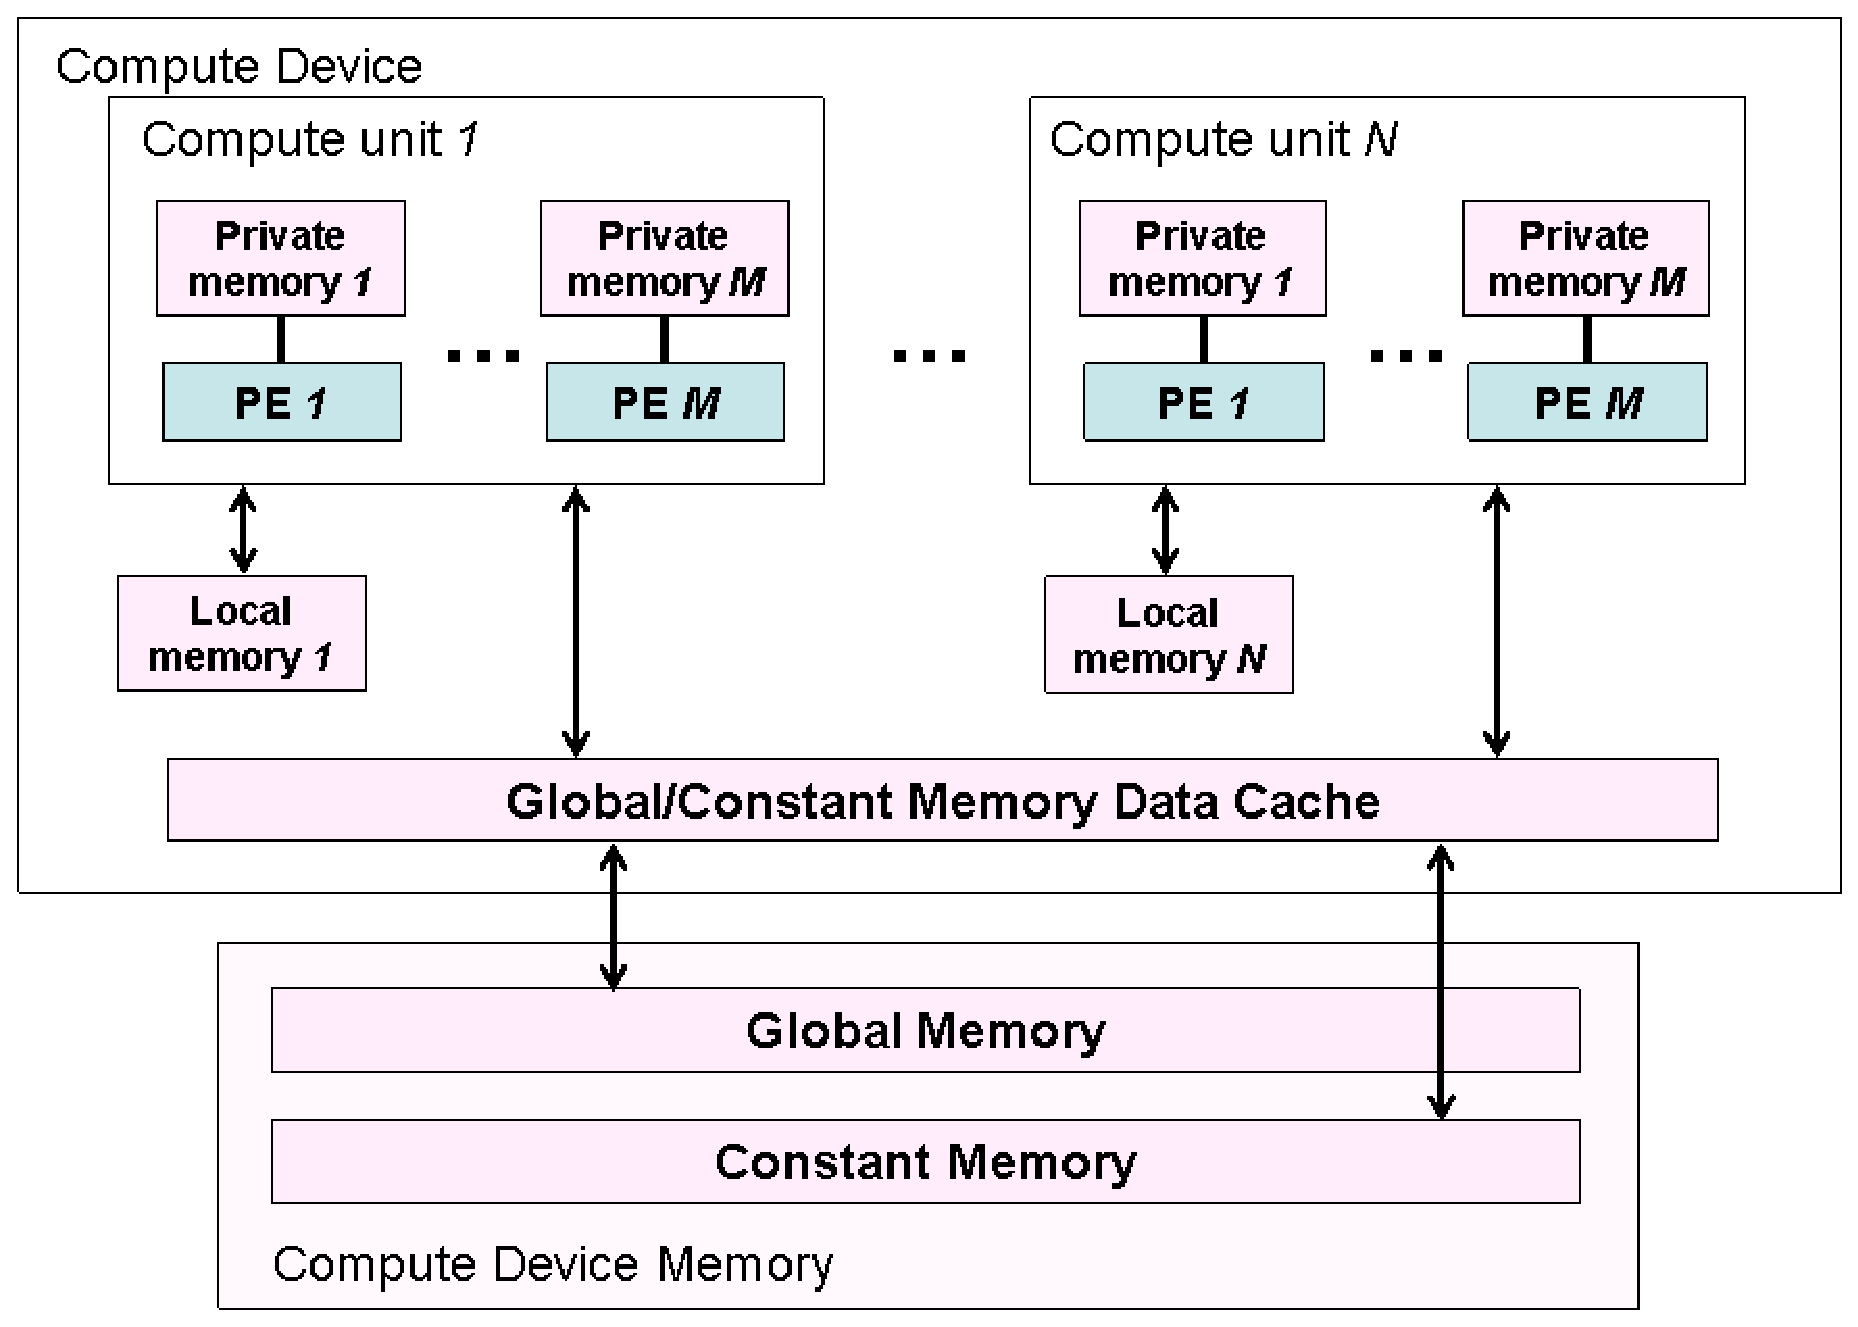
\includegraphics[width=0.6\columnwidth]{figures/eps/device.eps}
		\caption{OpenCL device architektúra (forrás: \cite{opencl})} 
		\label{fig:device} 
	\end{figure}
	
	
\section{OpenCL programozási modell}
	
	A programozási modell a hozzá tartozó osztálydiagrammon (\ref{fig:class}. ábra) figyelhető meg.
	
	\begin{figure}[!ht]
		\centering
		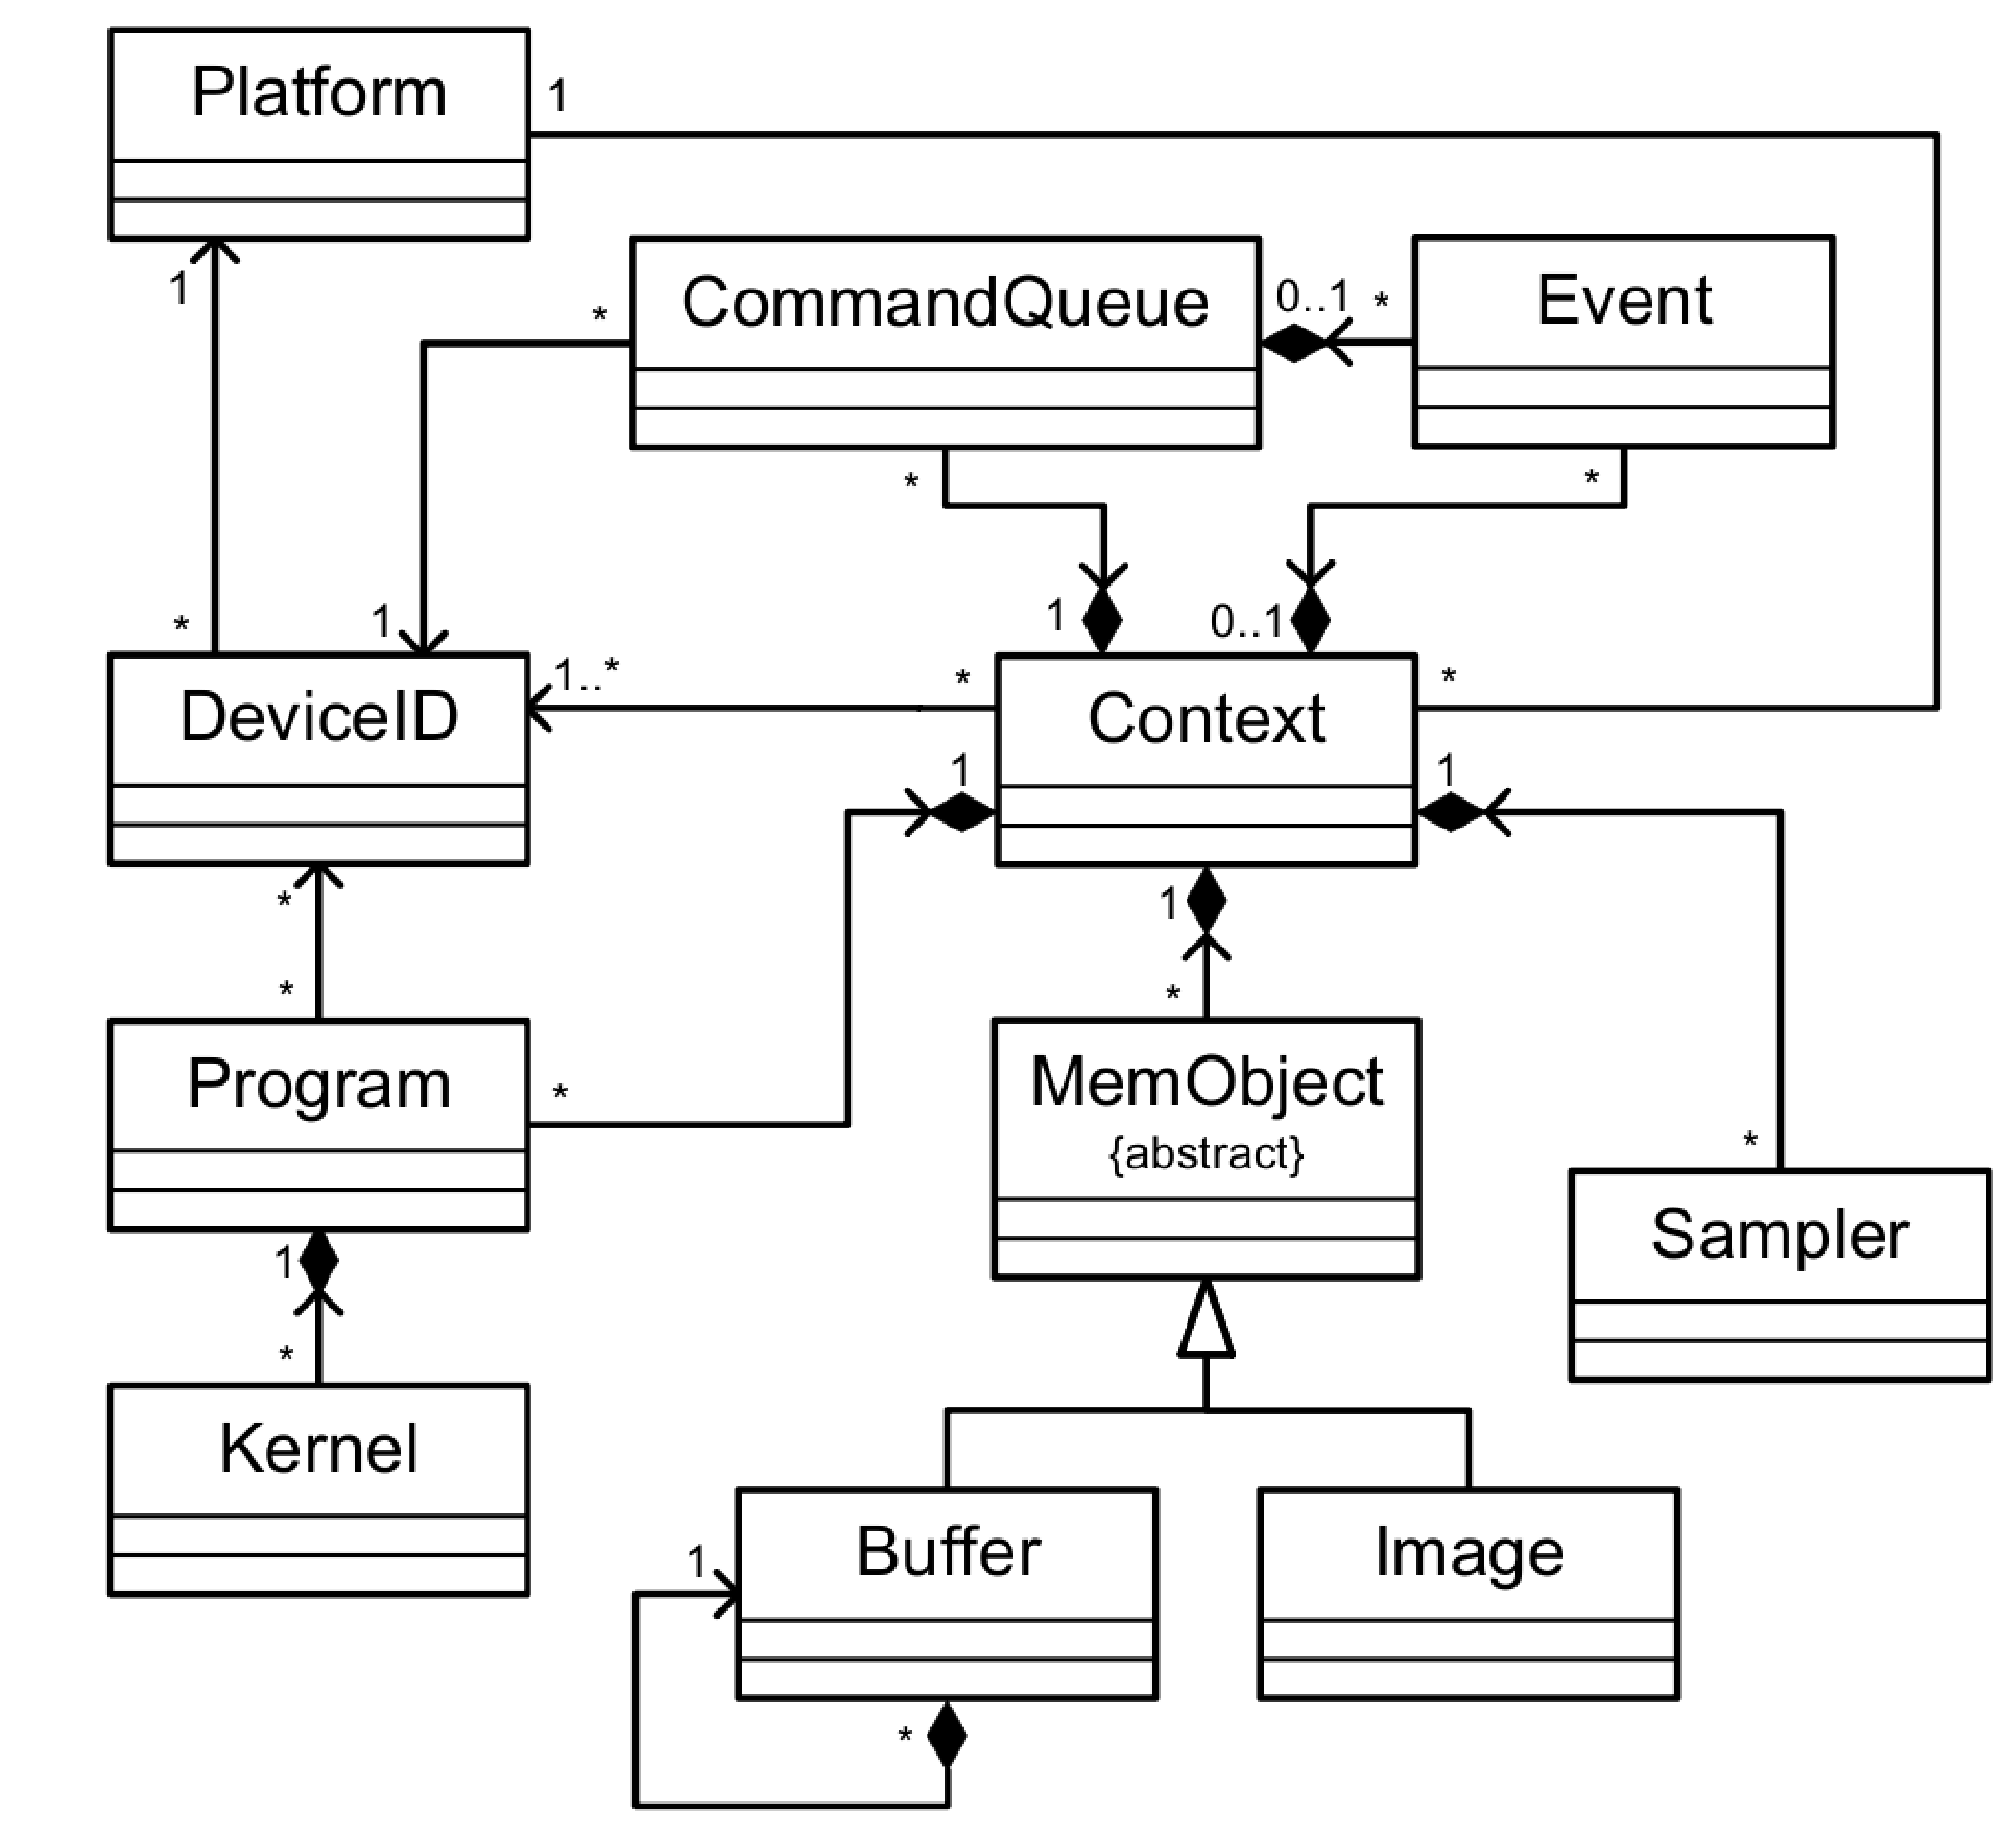
\includegraphics[width=0.6\columnwidth]{figures/eps/context.eps}
		\caption{OpenCL context osztálydiagrammja (forrás: \cite{opencl})} 
		\label{fig:class} 
	\end{figure}
	A futtatáshoz szükséges, hogy a kontextushoz platformot, majd azon belül
	eszközt, az eszközhöz programot (kernelt) és memóriát rendeljünk.
	Figyelembe kell vennünk azt a megkötést, hogy csak az egy platformon belüli
	eszközök programozhatóak heterogén módon. Például: Intel platform esetén
	lehetséges CPU-t, processzorkártyát és Intel-es GPU-t programozni, viszont nVidia kártyákat már nem.
	
	A programozással megoldandó problémát kétféleképpen lehetséges a feldolgozó
	egységekhez (work-item) avagy processzorokhoz rendelni:
	adat parallel módon vagy taszk parallel módon.
	
	Adat parallel módon (\ref{fig:data_parallel} ábra) a feldolgozandó adat egy
	részéhez rendelünk egy feldolgozó egységet. Fontos figyelembe venni az eszköz korlátos
	számú feldolgozó egységének számát. Ha nem elég a feldolgozó egysége akkor a
	feladat megfelelő partícionálásával lehetséges kordában tartani a szükséges
	erőforrás számát.
	
	Taszk parallel módot (\ref{fig:task_parallel} ábra) olyan esetben célszerű
	használna, ha a bemenet dinamikus mérete a futási időben rendkívül változik
	illetve a végrehajtandó feladat lazán függenek össze.
	
	\begin{figure*}[!ht]
		\centering
		\subfloat[Adat parallel]{
			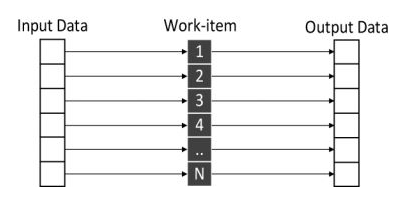
\includegraphics[width=0.45\columnwidth]{figures/eps/data.eps}%
			\label{fig:data_parallel}
		}
		\hfil
		\subfloat[Taszk parallel]{
			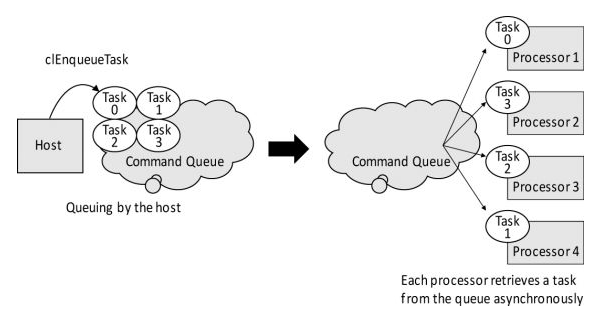
\includegraphics[width=0.45\columnwidth]{figures/eps/task.eps}%
			\label{fig:task_parallel}
		}
		\caption{Feladat hozzárendelése work-item-hez (processzorhoz)}
		\label{fig:parallel}
	\end{figure*}
	A processzor-magok megfelelő kihasználtságának elérése végett több ezer
	work-item virtuálisan osztozik rajta.
	Ezen work-item-eket work-group-okba rendezzük.
	\todo[prepend]{Írni a csoportbarendezés motivációjáró >> SIMD \& vector}
	A work-itemeket jelen pillanatban az OpenCL specifikációja \cite{opencl} szerint $3$ dimenziós
	work-group-ba tudjuk rendezni. Egy példát láthatunk egy work-item indexének a globális és lokális megfelelőjére a
	követekző \ref{fig:ndrange}. ábrán.
	
	\begin{figure}[!h]
		\centering
		\includegraphics[width=0.9\columnwidth]{figures/eps/ndrange.eps}
		\caption{2D-s work-item-ek work-group-ba rendezése és indexelése (forrás: \cite{opencl})} 
		\label{fig:ndrange} 
	\end{figure}
	
	
	Az OpenCL a fizikailag kialíkított memóriákat négy kategórába sorolja a tipikus memóriák kategorizálása a következők:
	\begin{itemize}
		\item \emph{Regiszterek:} Private memory,
		\item \emph{Chipen belüli memória (cache):} Local memory,
		\item \emph{Chipen kívüli memória:} Global memory és Constant Memory.
	\end{itemize}
	A privát és a lokális memória kis méretűnek és gyors elérésűnek mondható, míg a globális és konstans memória nagynak, de
	lassú elérésűnek.
	A definiált memória szintek tipikus paraméterei a következők:
	\begin{itemize}
	 	\item \emph{Privát memória:} minden szálnak külön van, amit a compiler menedzsel.
		\item \emph{Globális és konstans memória:}  Bank szervezés jellemző rá, gyors, de nagy késleltetéssel bír. 8 műveletet
		tud egy ciklus alatt végrehajtan, de csak a parancs kiadása után 400-800 ciklus késleltetéssel. Ha az adaton végrehajtandó
		műveletek ideje ennél jóval nagyobb, akkor ezt a késleltetést el lehet rejteni. 
		\item \emph{Lokális memória:} Minden work-group-nak sajátja van. Minimális a késletetés, sebessége nagy (38-44 GB/s).
		\item \emph{Host memória:} Nagy méretű, közepes sebességű, de sebességét a host-ot és a device-t összekötő PCIe interfész
		korlátozza.
	\end{itemize}
	A memóriákra megkötésként szolgál, hogy ki allokálhat, írhat és olvashat belőle. A \ref{table:mem}. táblázatban látható ezen
	jogosultságokat és a főbb tulajdonságokat.
	
	\begin{table}[!h]
	\renewcommand{\arraystretch}{1.3}
	% if using array.sty, it might be a good idea to tweak the value of
	% \extrarowheight as needed to properly center the text within the cells
	\caption{OpenCL memória szintek}
	\label{table:mem}
	\centering
	% Some packages, such as MDW tools, offer better commands for making tables
	% than the plain LaTeX2e tabular which is used here.
	\begin{tabular}{l|l|l|l|l}
			 & Host memory & Global memory & Local mem. & Private mem.\\ \hline
		Host & Dinamikusan R/W & Din. R/W &  Din. R/W & - \\
		Kernel & - & R/W & Satik. R/W & Statik. R/W\\
		Sebesség & Lassú & Közepes & Gyors & Regiszter\\
		Méret & $4$ Gb $\leq$ & $1$ Gb $\leq$ & $16,32$ Kb & $<1$ Kb
	\end{tabular}
	\end{table}

	A work-group-okba rendezés a lokális memória jogusultsága miatt érdekes.
	Konkrétan az egy work-group-ba tartozó összes work-item azonos lokális memórián
	osztozik.
	Ennek a következménye az, hogy adat parallel módú feldolgozás esetén
	az egymásra ható adatokhoz tartozó work-item-eket egy work groupba kell
	rendelnünk.
	Ha ez nem lehetséges, akkor a globális memóriához kell fordulnunk.
	A globális memória avagy a bank szervezésű külső (off-chip) memóriák
	hozzáférési ideje relatíve nagy így ezek használatát lehetőleg el kell kerülni
	és a programozónak kell ``cachelni" a lokális memóriába.
	
	Mivel a work-item-ek konkurrensen hajtódnak végre, így az általuk közösen elérhető memóriákra
	(globális, lokális) nézve versenyhelyzetben vannak.
	Az OpenCL ezt a problémát a laza memóriamodell használatával oldja meg.
	Work-item-ek közötti szinkronizációra egy korlátot alkalmaz a programban, amit csak akkor léphet át, ha az összes többi
	work-item (az azonos work-group-ban) ezt a korlátot már elérte.
	Erre a \texttt{barrier(FLAG)} függvényhívás szolgál. Fontos megjegyezni, hogy ez a szinkronizáció csak egy adott
	work-group-on belül történik, a work-group-ok közötti és akülönböző work-group-okon belüli work-item-ek szinkronizációra nincs
	lehetőség.
	
	\begin{center}
		Összefoglalva: nagy hangsúlyt kell a memóriaszervezésre fordítani, hogy a processzormagok megfelelően legyenek az adatokkal
		táplálva az elérhető számítási kapacitás kiaknázása végett.
	\end{center}


\section{Futási környezet bemutatása}
	A következő eszközök teljesítményét vizsgálom:
	\begin{itemize}
		\item A laptopomban található \textbf{Intel Core i5 M520} processzor,
		\item A laptopomban található kis teljesítményű \textbf{nVidia GT330M} videókártya,
% 		\item Asztali PC-ben található \textbf{Intel Xeon CPU},
% 		\item Asztali PC-ben található \textbf{Intel Xeon Phi} co-processzor \cite{phi,mic}. 
	\end{itemize}
	Ezen eszközök legjelentősebb paraméterei a \ref{table:envs} táblázat tartalmazza.
	
	\begin{table}[!ht]
	\renewcommand{\arraystretch}{1.3}
	% if using array.sty, it might be a good idea to tweak the value of
	% \extrarowheight  as needed to properly center the text within the cells
	\setlength{\extrarowheight}{8pt}
	\caption{Használandó eszközök összehasonlítása}
	\label{table:envs}
	\centering
	\footnotesize
	% Some packages, such as MDW tools, offer better commands for making tables
	% than the plain LaTeX2e tabular which is used here.
% 	\begin{tabular}{ l | r | r | r | r}
% 		 & Intel Core i5 & nVidia GT330M & Intel Xeon & Xeon PHI \\ \hline
% 		MAX COMPUTE UNITS & $4$ & $6$ & $8$ & $224$\\
% 		MAX CLOCK FREQUENCY & 2400 & 1265 & 3000 & 1100\\
% 		MAX WORK GROUP\_SIZE & $8192$ & $512$ & $8192$ & $8192$ \\ \hline\hline
% 		GLOBAL MEM SIZE & $\sim 4Gbyte$ & $1Gbyte$ & $8Gbyte$ & $\sim 4.5Gbyte$\\
% 		%MAX\_CONSTANT\_BUFFER\_SIZE & $131072$ & $65536$ & $131072$ & $131072$\\
% 		LOCAL MEM SIZE & $32 Kbyte$ & $16 Kbyte$ & $32 Kbyte$ & $32 Kbyte$\\
% 	\end{tabular}
	
	\begin{tabular}{ l | r | r}
		 & Intel Core i5 M520 & nVidia GT330M \\ \hline
		MAX COMPUTE UNITS & $4$ & $6$\\
		MAX CLOCK FREQUENCY & $2400$ MHz & $1265$ MHz \\
		MAX WORK GROUP\_SIZE & $8192$ & $512$ \\ \hline\hline
		GLOBAL MEM SIZE & $4GB\ (2GB)$ & $1GB\ (768 MB)$\\
		%MAX\_CONSTANT\_BUFFER\_SIZE & $131072$ & $65536$ & $131072$ & $131072$\\
		LOCAL MEM SIZE & $32 KB$ & $16 KB$\\
	\end{tabular}
	\end{table}
	
	Az összehasonlíthatóság végett a legkissebb memóriájú eszközre fogom a problémát skálázni, ami a
	GT330M videókártya. A CPU memóriája jóval nagyobb, így a kód mindegyiken tud futni.




